\documentclass{article}
\usepackage{forest}
\usepackage{tabularx}
\usepackage{amsmath}
\usepackage{float}
\usepackage{enumitem}
\usepackage{graphicx}
\usepackage{caption}
\usepackage{listings}
\usepackage{caption}
\usepackage{hyperref}

\UseRawInputEncoding

\lstset{
	language=Python,
	basicstyle=\ttfamily,
	breaklines=true,                % Enable line breaking
	breakatwhitespace=false,        % Line breaks at any character
}

\title{Final Summary: Anisotropic Diffusion - The Perona Malik PDE Applied}

\author{
	Alles Rebel \\
	MATH 693B Adv Computational PDE \\
	Professor Nguyen-Truc-Dao Nguyen
}

\begin{document}

\maketitle

\section*{Introduction}
Computer vision is rich with applications where edge detection is crucial for enabling computers to interpret the world. One notable application is Simultaneous Localization and Mapping (SLAM), where machines process a series of 2D images captured from sensors to perceive their own location and the surroundings. This capability is fundamental to autonomous systems and AR/VR applications, which require either comprehension of walls and their relative positions or the ability to avoid obstacles. We'll discuss these concepts, along with a Partial Differential Equation called the Perona Malik Equation \cite{perona1987scale}, and it's implementation as a finite difference scheme.

\section*{Background}
Most SLAM algorithms employ a pipeline that extracts features (e.g., perspective-invariant aspects or corners) from images, creates descriptors of these features, and matches them across various images as time progresses. Descriptors are methods that describe a feature using its local spatial information. By matching these feature descriptors and using a relative sensor such as an accelerometer, trajectories are constructed. Similar to the operation of a Kalman filter, the absolute sensor (the camera) is enhanced by the relative acceleration measurements provided by the accelerometer.

Edges further enhance this process by reducing error magnitudes over time. Edges are detected in the current image, and then a descriptor is generated along the edge. Instead of focusing solely at the feature point, an edge descriptor considers the area around the entire edge. Subsequent images then undergo the same matching procedure for any detected edges. Edges can be linked together, facilitating the generation of bounding boxes or even predicting occlusion.

\subsection*{How to Detect Edges}
Edge detection is one of the most extensively studied problems in computer vision. Edges can arise for various reasons, such as intensity variation, depth differences, or texture changes. The simplest approach to edge detection involves using a gradient, or a first-order derivative in the spatial direction of the image. As discussed in class, whenever we encounter a derivative, we can apply a partial difference scheme. Here, we use the forward difference operator to approximate the gradient, which is implemented via one of the most fundamental computer vision operations: 2D convolution filtering. If derivatives in both directions are needed, this can be achieved by convolving the respective kernels, as convolution is associative and commutative.

However, the first derivative is highly sensitive to noise. Every image captured by a sensor inherently contains noise, which can be amplified by this method. To address this, we often resort to the second derivative for detecting rapid intensity changes, known as the Laplacian. Using finite difference schemes, we can implement a first-order central difference approximation for the second derivative. This can be converted into a convolution kernel, which is a well-known kernel among computer vision students. The Laplacian kernel, which is central to this approach, is given by:
\[
\text{Laplacian Kernel} = \begin{bmatrix}
	0 & 1 & 0 \\
	1 & -4 & 1 \\
	0 & 1 & 0
\end{bmatrix}
\]
This kernel is used to detect areas of rapid intensity change in all directions in an image. 

Additionally, the Sobel operator, often used to calculate the gradient of the image intensity, uses two separate kernels to capture horizontal and vertical derivative approximations. The kernels are defined as:
\[
\text{Sobel Kernel X} = \begin{bmatrix}
	-1 & 0 & 1 \\
	-2 & 0 & 2 \\
	-1 & 0 & 1
\end{bmatrix},
\quad
\text{Sobel Kernel Y} = \begin{bmatrix}
	-1 & -2 & -1 \\
	0 & 0 & 0 \\
	1 & 2 & 1
\end{bmatrix}
\]
These kernels help in emphasizing edges that are vertically and horizontally oriented by computing the gradient in the X and Y directions, respectively.

Gradient calculations are at the heart of one of the most common edge detection algorithms: the Canny Edge Detector. In addition to gradient calculations, noise reduction methods are applied, along with thresholding of intensities, and edge tracking techniques. For the experiment below, we'll utilize the Canny Edge Detector, implemented using the standard accelerated convolutions provided by OpenCV and see the effect of applying Anisotropic Diffusion. 

\section*{Anisotropic Diffusion / Perona-Malik}
The value of edge detection and its challenges, such as the difficulty in distinguishing closely spaced edges or following a curve, lead to the development of methods like anisotropic diffusion. Perona and Malik applied the diffusive properties of the heat equation to the intensity values of an image's pixels, but restricted its application to areas not deemed edges. This method, known as anisotropic diffusion, smooths out the areas away from edges while preserving the edges themselves.

\subsection*{The PDE}
The Perona-Malik anisotropic diffusion is a partial differential equation (PDE) that modifies the image intensity as a function of both space and time. The PDE is given by:
\[
\frac{\partial I}{\partial t} = \nabla \cdot (c(\nabla I) \nabla I)
\]
where $I$ represents the image intensity, $\nabla I$ is the gradient of the intensity, and $c(\nabla I)$ is the diffusion coefficient that is a function of the intensity gradient.

\subsection*{The Finite Difference Scheme}
Perona and Malik proposed a finite difference scheme for approximating the above PDE, expressed as follows:
\[
I^{n+1}_{i,j} = I^n_{i,j} + \lambda \left[ c_{i+1,j} (I^n_{i+1,j} - I^n_{i,j}) + c_{i-1,j} (I^n_{i-1,j} - I^n_{i,j}) + c_{i,j+1} (I^n_{i,j+1} - I^n_{i,j}) + c_{i,j-1} (I^n_{i,j-1} - I^n_{i,j}) \right]
\]
where $\lambda$ is a time-step factor, and $c_{i,j}$ is the diffusion coefficient at pixel location $(i, j)$.

Stability analysis by the authors led to the condition:
\[
\lambda \leq \frac{1}{4}
\]

\subsection*{Intuition of Edge Preservation}
The intuition behind the edge preservation capability of the Perona-Malik scheme arises from several observations:
\begin{itemize}
	\item A correction term is added to the previous value of the pixel, which accounts for the local variations in intensity.
	\item The correction term incorporates the diffusion coefficient $c(\nabla I)$, which is calculated as:
	\[
	c(\nabla I) = e^{-\left(\frac{|\nabla I|^2}{K^2}\right)}
	\]
	where $K$ is a constant that controls the sensitivity of the diffusion process to edges.
	\item The diffusion coefficient $c(\nabla I)$ is designed to be small at edges (where the gradient $|\nabla I|$ is large), thus reducing diffusion across edges while allowing it in homogenous regions.
	\item This differential diffusion effectively preserves edges, as areas of high gradient undergo minimal smoothing, maintaining the sharpness and integrity of edges.
\end{itemize}
Note: The authors present two methods for implementing the correction term, both have the same intuition.

\section*{Example Results}
To demonstrate both the convolutional kernel method discussed earlier and the implementation of the Finite Difference scheme, a Python implementation utilizing OpenCV is shown in Appendix \ref{code-perona-malik}.

Utilizing the code, an input image is passed in via the command line when invoking the Python script, shown in Figure \ref*{fig:results}.
\
\begin{figure}[H]
	\centering
	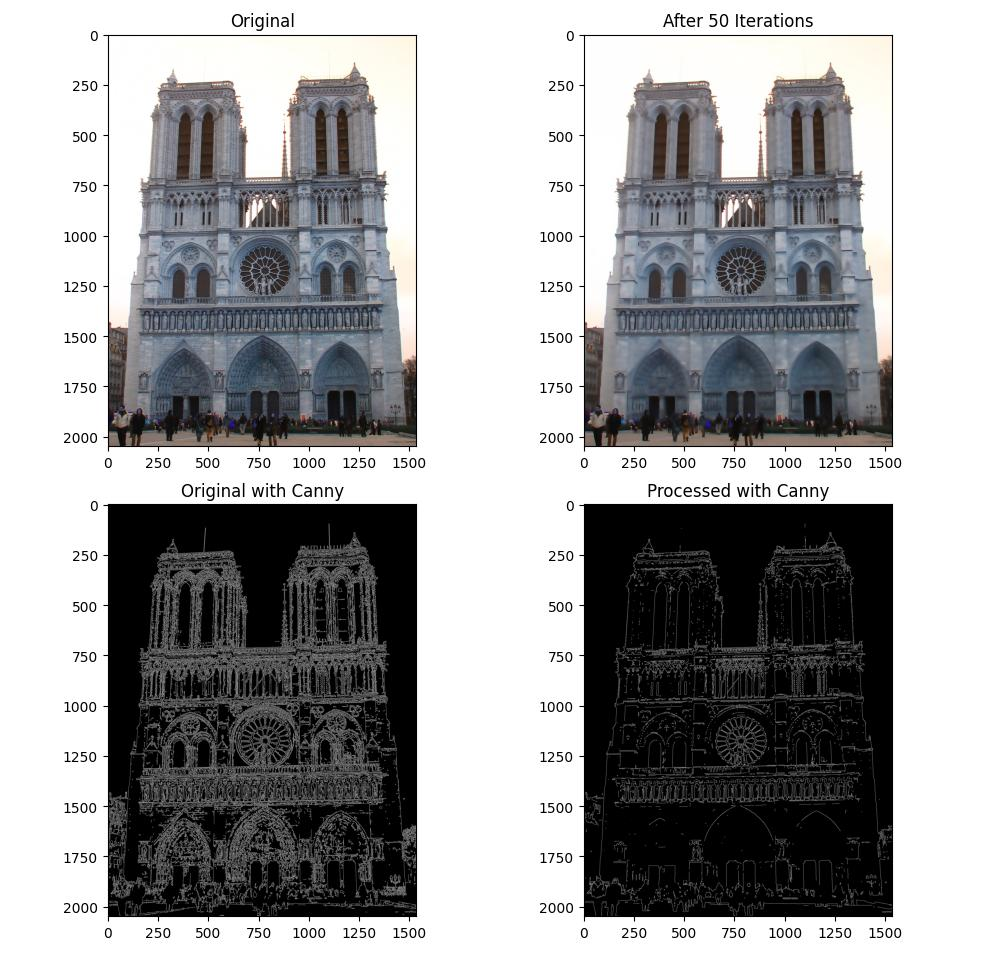
\includegraphics[width=\textwidth]{figureA.jpeg}
	\caption{Comparison of original and processed images. Top left: Original image. Top right: Image after 50 iterations of the Perona-Malik finite difference scheme. Bottom left: Canny edge detector applied to the original image. Bottom right: Canny edge detector applied to the processed image.}
	\label{fig:results}
\end{figure}

\section*{Conclusion}
Convolution kernels are a fundamental concept that nearly every computer science student encounters during their studies. However, the mathematical foundations often remain an afterthought. I have frequently used these kernels without realizing that they were actually implementations of a finite difference scheme, complete with the same stability constraints as any other finite difference scheme. In addition, utilizing standardized accelerated function calls significantly speed up computation, often an afterthought mathematical communities. 

\section*{Appendix}
All code written in python3.10, using matplot lib:
\subsection*{Reference Python Implementation} \label{code-perona-malik}
\lstinputlisting[language=Python]{PeronaMalik.py}

% Auto generates References Section
\bibliographystyle{ieeetr}
\bibliography{references.bib}

\end{document}